\documentclass[11pt]{beamer}  %% versione proiettore
%%\documentclass[11pt,handout]{beamer} %% versione stampa
\usepackage{lucidiJb-2ed}

\usepackage{relsize}

\mode<article>
{
  \usepackage{fullpage}
  \usepackage{hyperref}
}

\mode<presentation>
{
  \setbeamertemplate{background canvas}[vertical shading][bottom=red!10,top=blue!10]
  \usetheme{Ethereum}
  \usefonttheme[onlysmall]{structurebold}
}

\subtitle{Learning Ethereum}
\title{Smart Contracts}
\institute{Universit\`a di Verona, Italy}
\date{January 2020}

\setbeamercovered{invisible}

\def\codesize{\smaller}
\def\<#1>{\codeid{#1}}
\newcommand{\codeid}[1]{\ifmmode{\mbox{\codesize\ttfamily{#1}}}\else{\codesize\ttfamily #1}\fi}

\begin{document}

\begin{frame}
  \titlepage
\end{frame}

\begin{frame}\frametitle{A smart contract is\ldots}

  \begin{itemize}
  \item a computer program (not \emph{smart} nor \emph{a contract})
  \item immutable
  \item deterministic
  \item operating on restricted data
  \item running on a decentralized world computer
  \end{itemize}

  In Ethereum:
  \begin{itemize}
  \item compiled into EVM bytecode
  \item installed by sending a special transaction to address \<0x0>
  \item its code can be deleted if it contains a \<SELFDESTRUCT> bytecode
  \item has no keys
  \item who installs it gets no automatic privileges
  \item runs after a transaction initiated by an EOA
    \begin{itemize}
    \item or a chain of transactions initiated by an EOA
    \item no parallelism, no background processing
    \end{itemize}
  \item transactions are atomic
  \end{itemize}
  
\end{frame}

\begin{frame}\frametitle{Solidity}

  \begin{greenbox}{}
    There are many programming languages for Ethereum smart contracts,
    but Solidity is the de facto choice:
    \begin{itemize}
    \item imperative
    \item vaguely object-oriented
    \item in continuous evolution
    \item \alert{non}-strongly-typed
    \item unorthogonal features
    \end{itemize}
  \end{greenbox}

\end{frame}

\begin{frame}\frametitle{Back to our first Solidity example}
  \begin{center}
    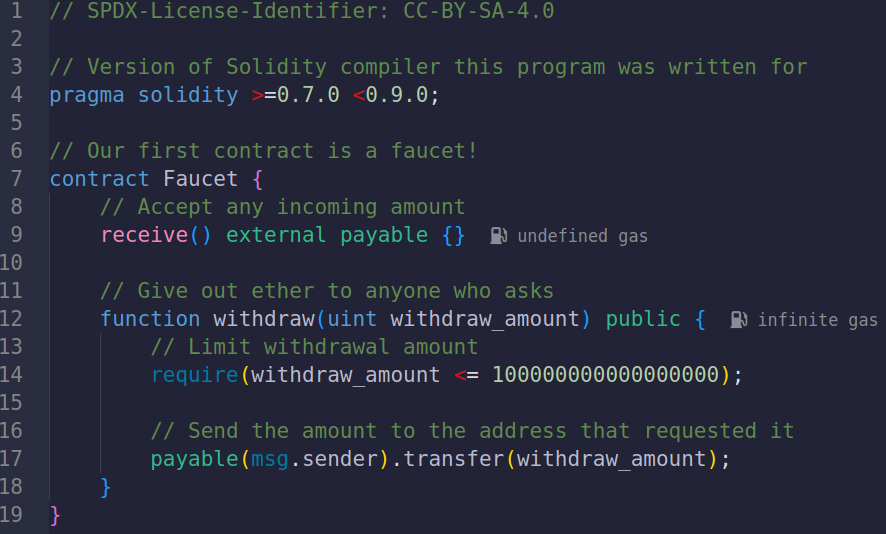
\includegraphics[width=\textwidth,clip=false]{pictures/faucet_sol.png}
  \end{center}
\end{frame}

\begin{frame}[fragile]\frametitle{ABI -- from Remix or from \<solc>}

{\scriptsize\begin{verbatim}
[
  {
    "payable": true,
    "stateMutability": "payable",
    "type": "fallback"
  },
  {
    "constant": false,
    "inputs": [
      {
        "internalType": "uint256",
        "name": "withdraw_amount",
        "type": "uint256"
      }
    ],
    "name": "withdraw",
    "outputs": [],
    "payable": false,
    "stateMutability": "nonpayable",
    "type": "function"
  }
]
\end{verbatim}}
\end{frame}

\begin{frame}[fragile]\frametitle{Select a compiler version}

  \begin{greenbox}{Add a pragma directive}
    \verb!pragma solidity ^0.4.19! requires to compile with a compiler for version $0.4.x$ with $x\ge 19$.
  \end{greenbox}

\end{frame}

\begin{frame}\frametitle{Basic Solidity types}
  \begin{greenbox}{\<bool>}
    with constants \<true> and \<false> and usual operators
  \end{greenbox}
  \bigskip
  \begin{greenbox}{\<int>, \<unint>}
    signed or unsigned, witgh usual operators, in increments of 8 bit size:
    \<uint8>, \<uint16>, \<int24>\ldots. Without specification, they stand for
    \<int256> and \<unint256>, respectively
  \end{greenbox}
  \bigskip
  \begin{greenbox}{\<fixed>$M\times N$, \<ufixed>$M\times N$}
    fixed point arithmetic, signed or unsigned, $M$ bits, $N$ decimals
    after th epoint
  \end{greenbox}
  \bigskip
  \begin{greenbox}{\<address>}
    a 20-bytes Ethereum address, with members \<balance> and \<transfer>
  \end{greenbox}

\end{frame}

\begin{frame}[fragile]\frametitle{Basic Solidity types}

  \begin{greenbox}{\<bytes>$N$}
    fixed-size array of bytes, of length $N$
  \end{greenbox}

  \bigskip

  \begin{greenbox}{\<bytes> or \<string>}
    variable-sized arrays of bytes
  \end{greenbox}

  \bigskip

  \begin{greenbox}{Arrays}
    \<uint32[][5]> is a fixed size array of five dynamic
    arrays of $32$ bits unsigned integers
  \end{greenbox}

  \bigskip

  \begin{greenbox}{Enum's}
\begin{verbatim}
enum NAME { A, B, ... }
\end{verbatim}
  \end{greenbox}

\end{frame}

\begin{frame}[fragile]\frametitle{Basic Solidity types}

  \begin{greenbox}{Struct's}
\begin{verbatim}
struct pair {
  int16 x;
  unint8 y;
}
\end{verbatim}
  \end{greenbox}

  \bigskip

  \begin{greenbox}{Mappings}
\begin{verbatim}
mapping(address => unint256) balances;
\end{verbatim}
  \end{greenbox}

\end{frame}

\begin{frame}[fragile]\frametitle{Unit multipliers}

  \begin{greenbox}{Time units: \<seconds>, \<minutes>, \<hours>, \<days>}
\begin{verbatim}
uint delay = 3 hours;
\end{verbatim}
  \end{greenbox}

  \bigskip

  \begin{greenbox}{Ether units: \<wei>, \<finney>, \<szabo>, \<ether>}
\begin{verbatim}
require(withdraw_amount <= 0.1 ether);
\end{verbatim}
  \end{greenbox}

\end{frame}

\begin{frame}\frametitle{Transaction information}

  \begin{greenbox}{Structures \<msg> and \<tx> are computed from the transaction request}
    \begin{description}
    \item[\<msg.sender>] the address that sent the transaction
    \item[\<msg.value>] the ether sent along the transaction
    \item[\<msg.gasleft>] what remains to consume of the gas limit
    \item[\<msg.data>] the data payload of the transaction
    \item[\<msg.sig>] the first four bytes of \<msg.data> (method selector)
    \item[\<tx.gasprice>] the gas price used
    \item[\<tx.origin>] the address of the \alert{originating} EOA
    \end{description}
  \end{greenbox}

\end{frame}

\begin{frame}\frametitle{\<msg.sender> vs \<tx.origin>}

  \begin{center}
    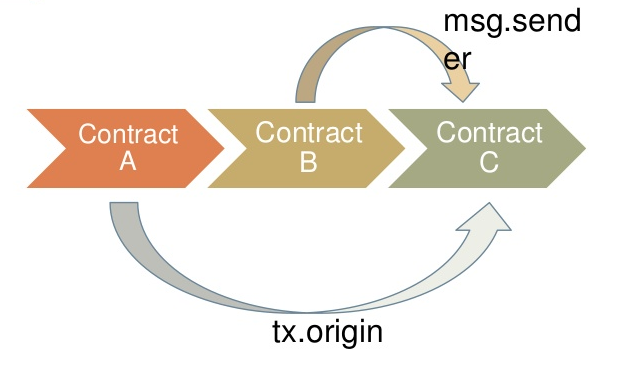
\includegraphics[width=\textwidth,clip=false]{pictures/sender-origin.png}
  \end{center}

\end{frame}

\begin{frame}\frametitle{Block information}

  \begin{greenbox}{The structure \<block> is constructed by the miner}
    \begin{description}
    \item[\<block.coinbase>] the address of the miner
    \item[\<block.difficulty>] the proof of work difficult
    \item[\<block.gaslimit>] the maximum gas spent in the block
    \item[\<block.number>] the current block height
    \item[\<block.timestamp>] the mining time
    \end{description}
  \end{greenbox}

\end{frame}
\begin{frame}\frametitle{Members of an address}

  \begin{greenbox}{}
    \begin{description}
    \item[\<address.balance>] the balance of the address (EOA or contract),
      such as \<address(this).balance>
    \item[\<address.transfer(x)>] sends $x$ wei to the address; throws an exception in case of
      failure
    \item[\<address.send(x)>] as \<transfer>, but returns \<false> in case of failure
    \item[\<address.call(p)>] sends a method transaction to the address, with the given
      payload; returns \<false> in case of failure
    \item[\<address.callcode(p)>] sends a method transaction to the address, with the given
      payload; runs in the scope of the caller; returns \<false> in case of failure
    \item[\<address.delegatecode(p)>] sends a method transaction to the address, with the given
      payload, but keeps \<msg.sender> and \<msg.value> unchanged;
      runs in the scope of the caller; returns \<false> in case of failure
    \end{description}
  \end{greenbox}
  
\end{frame}

\begin{frame}\frametitle{Main types in Solidity}

  \begin{description}
  \item[\<contract>] somehow similar to an object in OO-programming. It has a balance
  \item[\<interface>] functions have no code and must be implemented in subtypes
  \item[\<library>] a contract meant to be deployed once and used by other contracts through \<delegatecall>. It has no variables and no balance. It does not receive ether
    \begin{center}
      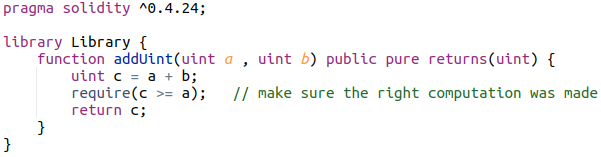
\includegraphics[scale=0.45,clip=false]{pictures/library.png}
    \end{center}
  \end{description}
  
\end{frame}

\begin{frame}\frametitle{Visibility modifiers}
  \begin{description}
  \item[\<public>] can be called from everywhere
  \item[\<external>] like \<public> but, if called from the same contract,
    must be prefixed with \<this.>. They cost less gas than \<public>
  \item[\<internal>] can only be called from the contract where they are defined
    or from its subtypes
  \item[\<private>] can only be called from the contract where they are defined
  \end{description}

  \bigskip

  \begin{redbox}{Privacy?}
    Data is always publicly readable in blockchain. These modifiers
    only refer to who can call whom.
  \end{redbox}
\end{frame}

\begin{frame}\frametitle{Side-effect modifiers}

  \begin{description}
  \item[\<view>] the function cannot modify the state
    \begin{center}
      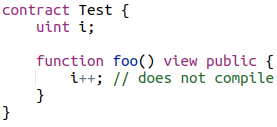
\includegraphics[scale=0.45,clip=false]{pictures/not-view.png}
    \end{center}
  \item[\<pure>] the function cannot modify nor read the state
    \begin{center}
      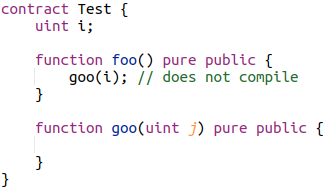
\includegraphics[scale=0.45,clip=false]{pictures/not-pure.png}
    \end{center}
  \item[\<payable>] the function can receive incoming payments
  \end{description}

\end{frame}

\begin{frame}\frametitle{Constructors}
  \begin{greenbox}{}
    A contract \alert{can} have \alert{up to one} contructor, that gets called
    only once as part of a transaction that deploys an instance
    of the contract.
  \end{greenbox}

  \begin{center}
    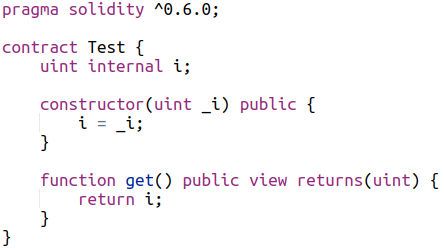
\includegraphics[scale=0.55,clip=false]{pictures/constructor.png}
  \end{center}

\end{frame}

\begin{frame}\frametitle{Self destruction example}

  Only needed to free state data in clients!

  \begin{center}
    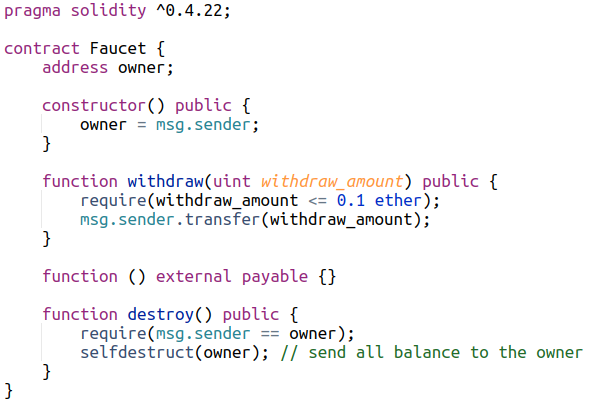
\includegraphics[scale=0.5,clip=false]{pictures/selfdestruct.png}
  \end{center}

\end{frame}

\begin{frame}\frametitle{Self destruction example from 0.6.0}

  \begin{center}
    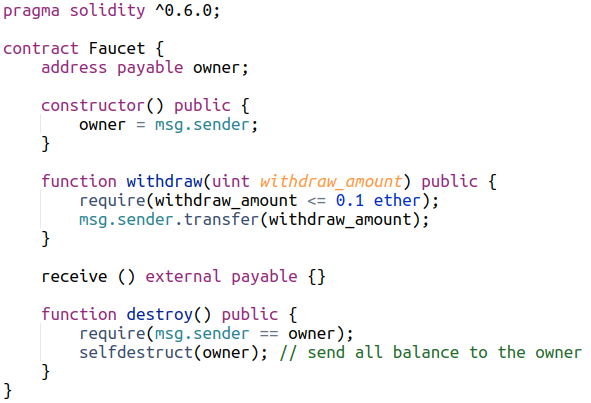
\includegraphics[scale=0.5,clip=false]{pictures/selfdestruct_6_0.png}
  \end{center}

\end{frame}

\begin{frame}\frametitle{\<address payable>}

  \begin{greenbox}{Starting from 0.5.0, an \<address> can be \<payable>}
    \begin{itemize}
    \item required for calling \<send()>, \<transfer()> and \<call()>
    \item all of \<msg.sender>, \<tx.origin> and \<block.coinbase> are
      \<payable>
    \item you can cast between \<address> and \<address payable> and such casts never fails
    \end{itemize}
  \end{greenbox}

  \bigskip

  \begin{greenbox}{Starting from 0.6.0, a contract can have at most
      a \<receive> function}
    \begin{itemize}
    \item it must be \<external payable>
    \item called for transactions without data
    \end{itemize}
  \end{greenbox}

  \bigskip

  \begin{greenbox}{Starting from 0.6.0, a contract can have at most
      a \<fallback> function}
    \begin{itemize}
    \item it must be \<external>
    \item called for transactions with data targetting no function in the
      contract or for transactions without data if there is no \<receive>
      function
    \end{itemize}
  \end{greenbox}

\end{frame}

\begin{frame}\frametitle{Modifiers}

  \begin{greenbox}{They can be used to weave aspects into code}
    \begin{center}
      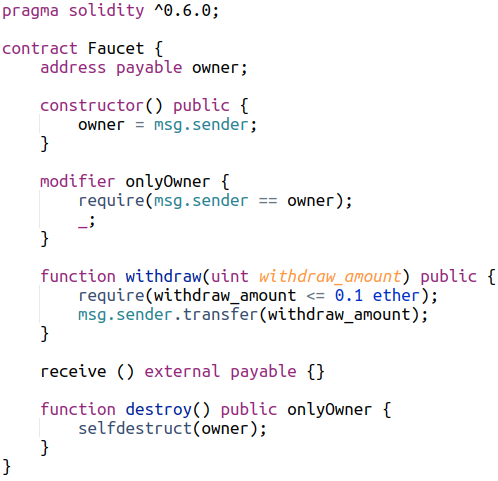
\includegraphics[scale=0.4,clip=false]{pictures/modifier.png}
    \end{center}
  \end{greenbox}

\end{frame}

\begin{frame}\frametitle{Modifiers}

  \begin{greenbox}{They can be used to do rather wierd things}
    \begin{center}
      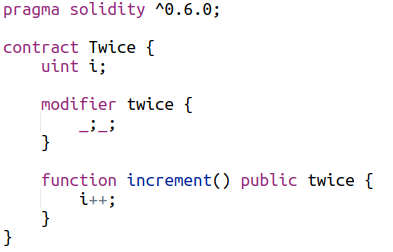
\includegraphics[scale=0.6,clip=false]{pictures/twice.png}
    \end{center}
  \end{greenbox}

\end{frame}

\begin{frame}\frametitle{Contract extension}

  \begin{greenbox}{}
    \begin{center}
      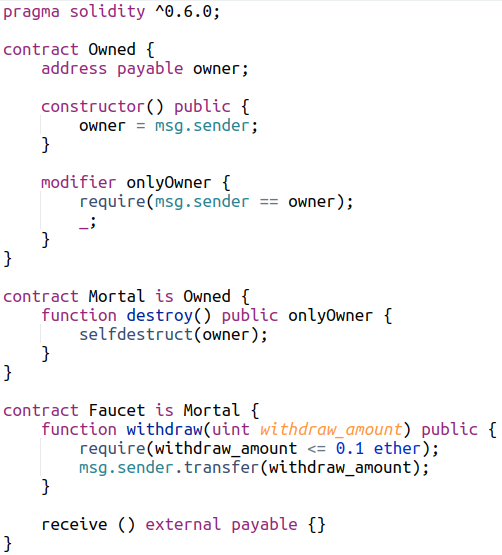
\includegraphics[scale=0.38,clip=false]{pictures/subcontracts.png}
    \end{center}
  \end{greenbox}

\end{frame}

\begin{frame}\frametitle{Constructor chaining}

  \begin{greenbox}{}
    \begin{center}
      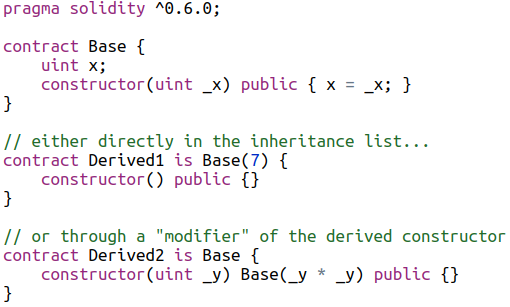
\includegraphics[width=\textwidth,clip=false]{pictures/constructor_chaining.png}
    \end{center}
  \end{greenbox}

\end{frame}

\begin{frame}\frametitle{Assertions}
  \begin{greenbox}{\<require(condition[,msg])>}
    Evaluates the condition. If false, an exception is thrown and the
    transaction is reverted. Typically used for checking function parameters.
  \end{greenbox}

  \bigskip

  \begin{greenbox}{\<assert(condition[,msg])>}
    Evaluates the condition, \alert{that is expected to hold}.
    If false, an exception is thrown and the
    transaction is reverted. Typically used to verify runtime conditions
    for debugging.
  \end{greenbox}

  \bigskip

  \begin{greenbox}{\<revert([msg])>}
    Throws an exception and reverts the current transaction.
  \end{greenbox}

  \bigskip

  \begin{redbox}{}
    There is no way to catch exceptions.
  \end{redbox}

\end{frame}

\begin{frame}\frametitle{Events}

  \begin{greenbox}{}
    \begin{center}
      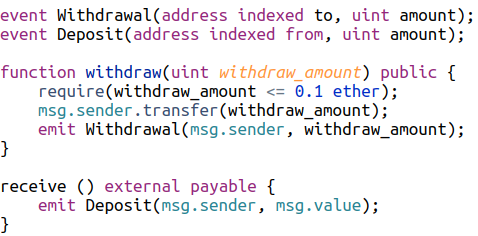
\includegraphics[width=\textwidth,clip=false]{pictures/events.png}
    \end{center}
  \end{greenbox}

  \bigskip

  DApps can listen and react to events.
\end{frame}

\begin{frame}\frametitle{Specifying gas and value for inner transactions}

  \begin{greenbox}{\<o.foo(pars)> can be decorated}
    \begin{itemize}
    \item \<o.foo.value(v)(pars)>
    \item \<o.foo.gas(g)(pars)>
    \item \<o.foo.gas(g).value(v)(pars)>
    \end{itemize}
  \end{greenbox}

  \bigskip

  \begin{greenbox}{\<new C(pars)> can be decorated}
    \begin{itemize}
    \item \<(new C).value(v)(pars)>
    \item \<(new C).gas(g)(pars)>
    \item \<(new C).gas(g).value(v)(pars)>
    \end{itemize}
  \end{greenbox}

\end{frame}

\begin{frame}\frametitle{Contract creation and function calls}

  \begin{greenbox}{}
    \begin{center}
      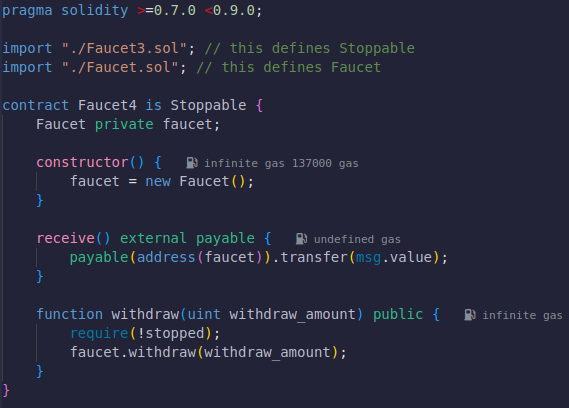
\includegraphics[scale=0.55,clip=false]{pictures/new-contract.png}
    \end{center}
  \end{greenbox}

  \bigskip

  We know what gets called with \<faucet.destroy()>.
\end{frame}

\begin{frame}\frametitle{Contract creation with payable constructor}

  \begin{greenbox}{If the constructor of \<Faucet> were made \<payable>}
    \begin{center}
      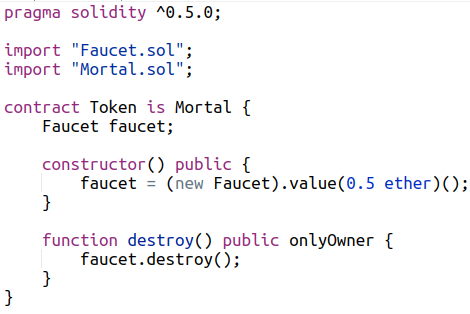
\includegraphics[scale=0.5,clip=false]{pictures/new-contract-payable.png}
    \end{center}
  \end{greenbox}

  \bigskip

  We know what gets called with \<faucet.destroy()>.
\end{frame}

\begin{frame}\frametitle{Casts do not fail in Solidity}

  \begin{center}
    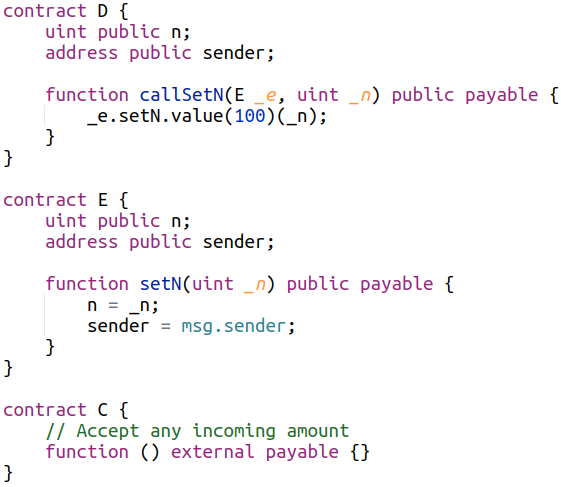
\includegraphics[scale=0.45,clip=false]{pictures/cast-does-not-fail.png}
  \end{center}

  Calling \<d.callFoo(c)>, where \<c> is a \<C>,
  does not fail but calls \<C>'s
  fallback function and transfers $100$ wei to \<c>!
\end{frame}

\begin{frame}\frametitle{Parameter contract types are just casts}

  \begin{center}
    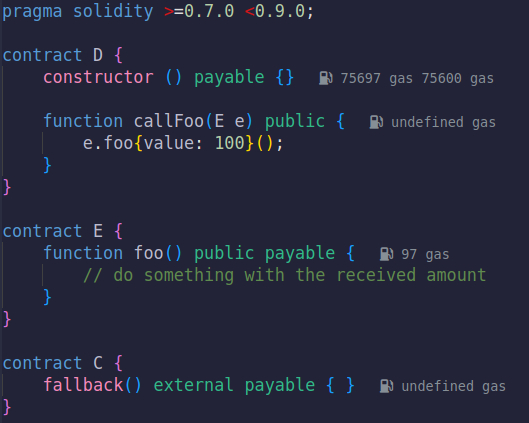
\includegraphics[scale=0.45,clip=false]{pictures/cast-does-not-fail2.png}
  \end{center}

  Calling \<d.callFoo(c)>, where \<c> is a \<C>,
  does not fail but calls \<C>'s
  fallback function and transfers $100$ wei to \<c>!
\end{frame}

\begin{frame}\frametitle{Solidity is \alert{not} strongly-typed}

  \begin{enumerate}
  \item Casts are not checked
  \item Parameter types are just Christmas decorations
  \end{enumerate}

  \bigskip

  \begin{redbox}{}
    Remember that a function declaring a formal parameter of type
    \<address> or explicitly \<C> can actually receive any contract, of any
    type, also completely unrelated to \<C>.
    Callers can inject malicious code through such parameters!
  \end{redbox}

  \begin{center}
    
\includegraphics[scale=0.28,clip=false]{pictures/frightened-cat.jpg}
  \end{center}

\end{frame}

\begin{frame}\frametitle{Members of an address for low-level calls}

  \begin{greenbox}{}
    \begin{description}
    \item[\<address.call(p)>] sends a method transaction to the address, with the given
      payload; returns \<false> in case of failure. This is actually used
      by the compiler when we write normal function calls
    \item[\<address.callcode(p)>] sends a method transaction to the address, with the given
      payload; runs in the scope of the caller; returns \<false> in case of failure
    \item[\<address.delegatecode(p)>] sends a method transaction to the address, with the given
      payload, but keeps \<msg.sender> and \<msg.value> unchanged;
      runs in the scope of the caller; returns \<false> in case of failure
    \end{description}
  \end{greenbox}
  
\end{frame}

\begin{frame}\frametitle{Example of function call}
  \begin{center}
    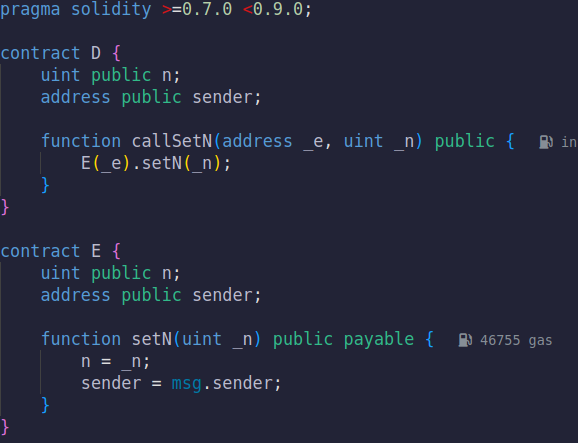
\includegraphics[scale=0.35,clip=false]{pictures/normal-call.png}
  \end{center}

  Calling \<d.callSetN(e, 42)>:
  \begin{itemize}
  \item \<e.n> will become $42$
  \item \<e.sender> will become \<d>
  \item \<d.n> and \<d.sender> are not modified
  \end{itemize}
\end{frame}

\begin{frame}\frametitle{The previous example is actually compiled into this}

  \begin{center}
    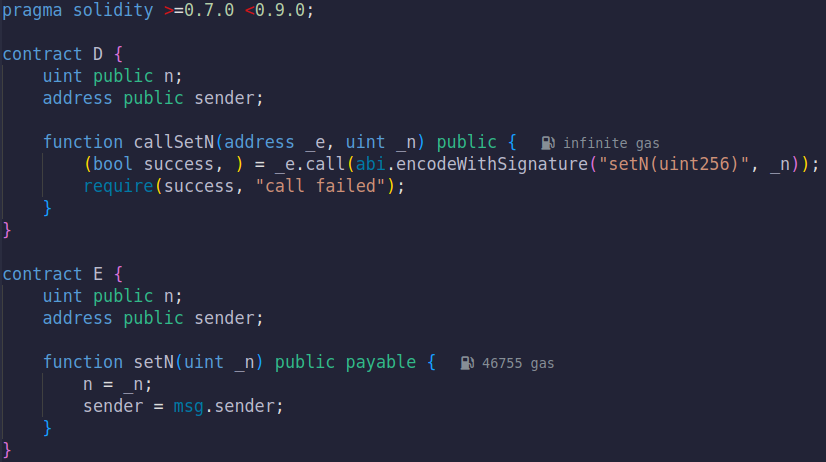
\includegraphics[scale=0.35,clip=false]{pictures/call.png}
  \end{center}

  Calling \<d.callSetN(e, 42)>:
  \begin{itemize}
  \item \<e.n> will become $42$
  \item \<e.sender> will become \<d>
  \item \<d.n> and \<d.sender> are not modified
  \end{itemize}
  
\end{frame}

%\begin{frame}\frametitle{Example of a failing low-level \<call>}

%  \begin{center}
%    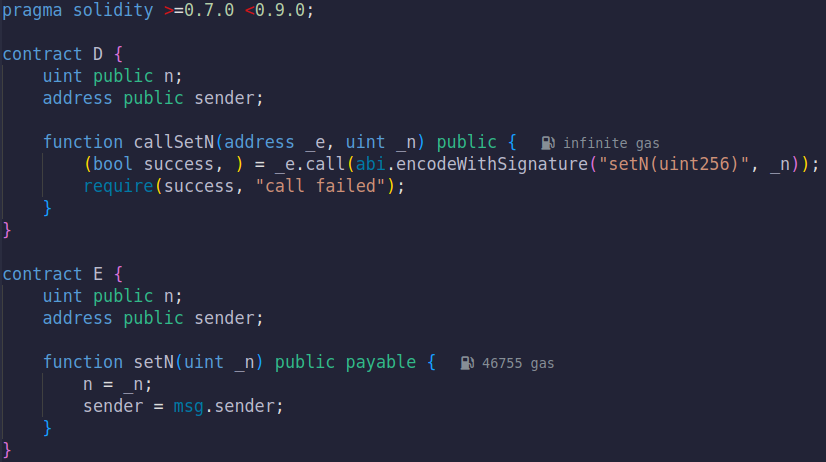
\includegraphics[scale=0.35,clip=false]{pictures/call.png}
%  \end{center}

%  Calling \<d.callSetN(c, 42)> where \<c> has no \<setN(uint \_n)> function:
%  \begin{itemize}
%  \item the outer transaction will succeed
%  \item the inner \<\_e.call> transaction will fail and be reverted
%  \item function \<\_e.call> will return \<false>
%  \end{itemize}
  
%\end{frame}

\begin{frame}\frametitle{Example of low-level \<callcode>}

  \begin{center}
    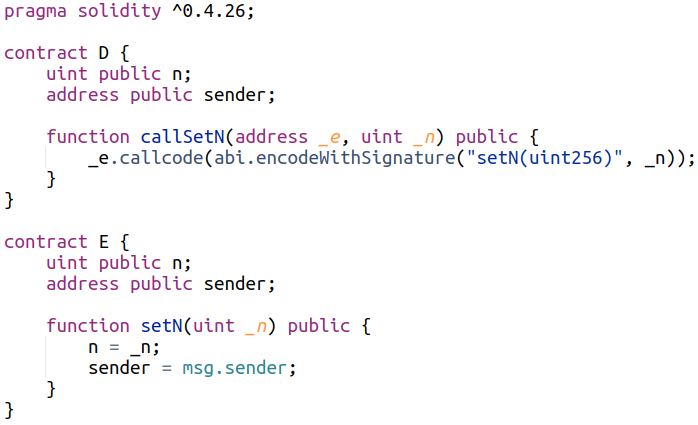
\includegraphics[scale=0.35,clip=false]{pictures/callcode.png}
  \end{center}

  Calling \<d.callSetN(e, 42)>:
  \begin{itemize}
  \item \<d.n> will become $42$
  \item \<d.sender> will become \<d>
  \item \<e.n> and \<e.sender> are not modified
  \end{itemize}
  
\end{frame}

\begin{frame}\frametitle{Example of low-level \<delegatecall>}

  \begin{center}
    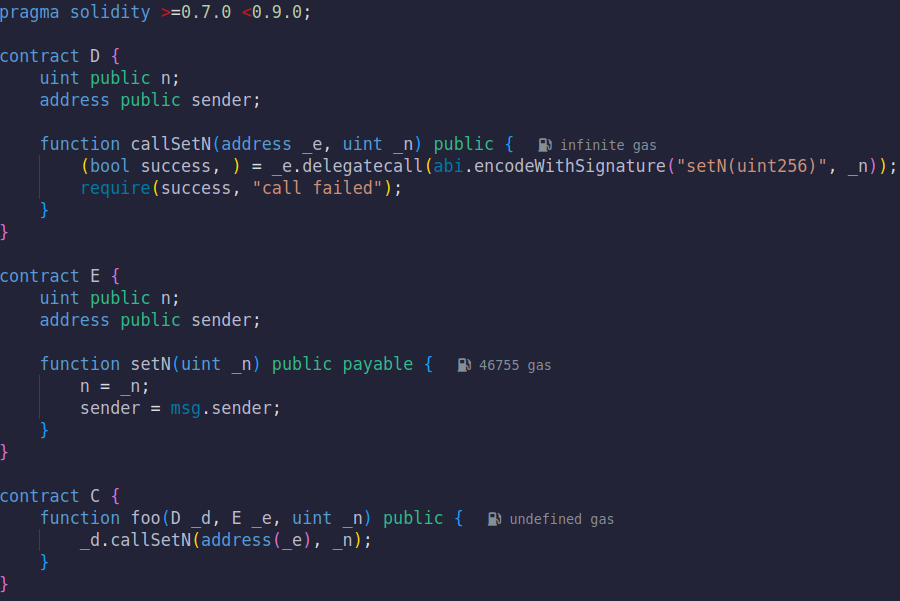
\includegraphics[scale=0.3,clip=false]{pictures/delegatecall.png}
  \end{center}

  Calling \<c.foo(d, e, 42)>:
  \begin{itemize}
  \item \<d.n> will become $42$
  \item \<d.sender> will become \<c>
  \item \<e.n> and \<e.sender> are not modified
  \end{itemize}
  
\end{frame}

\begin{frame}\frametitle{Gas consumption}

  \begin{greenbox}{Each bytecode instruction and transaction type has a gas cost}
    \begin{itemize}
    \item it is possible to estimate the gas cost of simple functions
      (use \<estimateGas> of web3 for instance)
    \item \alert{the estimation is wrong in the presence of loops or recursion!}
    \item in general, it is important to know which operations (might) cost much gas, to avoid them
      \begin{itemize}
      \item loops over unbounded dynamic arrays
      \item calls to unknown contracts
      \end{itemize}
    \end{itemize}
  \end{greenbox}
\end{frame}

\end{document}
